\documentclass[aps,twocolumn,secnumarabic,balancelastpage,amsmath,amssymb,nofootinbib]{revtex4}
% \documentclass[aps,twocolumn,secnumarabic,balancelastpage,amsmath,amssymb,nofootinbib]{revtex4}

% Documentclass Options

% nobalancelastpage doesn't attempt to equalize the lengths of the two columns
% on the last page as might be desired in a journal where articles follow one
% another closely
% amsmath and amssymb are necessary for the subequations environment among
% others secnumarabic identifies sections by number to aid electronic review
% and commentary. nofootinbib forces footnotes to occur on the page where they
% are first referenced and not in the bibliography

% \usepackage{lgrind}        % convert program listings to a form includable in a LaTeX document
\usepackage{chapterbib}    % allows a bibliography for each chapter (each labguide has it's own)
\usepackage{color}         % produces boxes or entire pages with colored backgrounds
\usepackage{graphics}      % standard graphics specifications
\usepackage[pdftex]{graphicx}      % alternative graphics specifications
\usepackage{longtable}     % helps with long table options
\usepackage{epsf}          % old package handles encapsulated post script issues
\usepackage{bm}            % special 'bold-math' package
\usepackage{tikz}
\usepackage{asymptote}     % For typesetting of mathematical illustrations
\usepackage{subfigure}

% \usepackage{thumbpdf}

\usepackage[colorlinks=true]{hyperref}  % this package should be added after all others
% use as follows: \url{http://web.mit.edu/8.13}
\newcommand{\drelectron}[1]{\node at #1 [circle, draw, inner sep=0pt, minimum size=1pt] {\_}}
\newcommand{\ud}{\mathrm{d}}
\newcommand{\ue}{\mathrm{e}}
\newcommand{\ui}{\mathrm{i}}
\newcommand{\res}{\mathrm{Res}}
\newcommand{\Tr}{\mathrm{Tr}}
\newcommand{\dsum}{\displaystyle\sum}
\newcommand{\dprod}{\displaystyle\prod}
\newcommand{\dlim}{\displaystyle\lim}
\newcommand{\dint}{\displaystyle\int}
\newcommand{\fsno}[1]{{\!\not\!{#1}}}
\newcommand{\eqar}[1]
{
  \begin{align*}
    #1
  \end{align*}
}
\newcommand{\texp}[2]{\ensuremath{{#1}\times10^{#2}}}
\newcommand{\dexp}[2]{\ensuremath{{#1}\cdot10^{#2}}}
\newcommand{\eval}[2]{{\left.{#1}\right|_{#2}}}
\newcommand{\paren}[1]{{\left({#1}\right)}}
\newcommand{\lparen}[1]{{\left({#1}\right.}}
\newcommand{\rparen}[1]{{\left.{#1}\right)}}
\newcommand{\abs}[1]{{\left|{#1}\right|}}
\newcommand{\sqr}[1]{{\left[{#1}\right]}}
\newcommand{\crly}[1]{{\left\{{#1}\right\}}}
\newcommand{\angl}[1]{{\left\langle{#1}\right\rangle}}
\newcommand{\tpdiff}[4][{}]{{\paren{\frac{\partial^{#1} {#2}}{\partial {#3}{}^{#1}}}_{#4}}}
\newcommand{\tpsdiff}[4][{}]{{\paren{\frac{\partial^{#1}}{\partial {#3}{}^{#1}}{#2}}_{#4}}}
\newcommand{\pdiff}[3][{}]{{\frac{\partial^{#1} {#2}}{\partial {#3}{}^{#1}}}}
\newcommand{\diff}[3][{}]{{\frac{\ud^{#1} {#2}}{\ud {#3}{}^{#1}}}}
\newcommand{\psdiff}[3][{}]{{\frac{\partial^{#1}}{\partial {#3}{}^{#1}} {#2}}}
\newcommand{\sdiff}[3][{}]{{\frac{\ud^{#1}}{\ud {#3}{}^{#1}} {#2}}}
\newcommand{\tpddiff}[4][{}]{{\left(\dfrac{\partial^{#1} {#2}}{\partial {#3}{}^{#1}}\right)_{#4}}}
\newcommand{\tpsddiff}[4][{}]{{\paren{\dfrac{\partial^{#1}}{\partial {#3}{}^{#1}}{#2}}_{#4}}}
\newcommand{\pddiff}[3][{}]{{\dfrac{\partial^{#1} {#2}}{\partial {#3}{}^{#1}}}}
\newcommand{\ddiff}[3][{}]{{\dfrac{\ud^{#1} {#2}}{\ud {#3}{}^{#1}}}}
\newcommand{\psddiff}[3][{}]{{\frac{\partial^{#1}}{\partial{}^{#1} {#3}} {#2}}}
\newcommand{\sddiff}[3][{}]{{\frac{\ud^{#1}}{\ud {#3}{}^{#1}} {#2}}}

\begin{document}
\tikzstyle{every picture}+=[remember picture]
\title{Non-linear effect and patterns in the scatterred beam of close resonance laser in a Rubidium vapor cell}
\author{Yichao Yu}
\email{yuyichao@mit.edu}
\homepage{http://yyc-arch.org/}
\date{\today}
\affiliation{MIT Department of Physics}

\begin{abstract}
\end{abstract}

\maketitle
%%%%%%%%%%%%%%%%%%%%%%%%%%%%%%%%%%%%%%%%%%%%%%%%%%%%%%%%%%%%%%%%%%
\section*{Introduction}

\section{Theory}
\subsection{Saturated absorption and non-linear effect.}
\subsection{Scattering in a standing wave and interference rings.}
\subsection{Flower like patterns from four wave mixing.}

\section{Apparatus}
\subsection{Beam path setup.}
\begin{figure}
  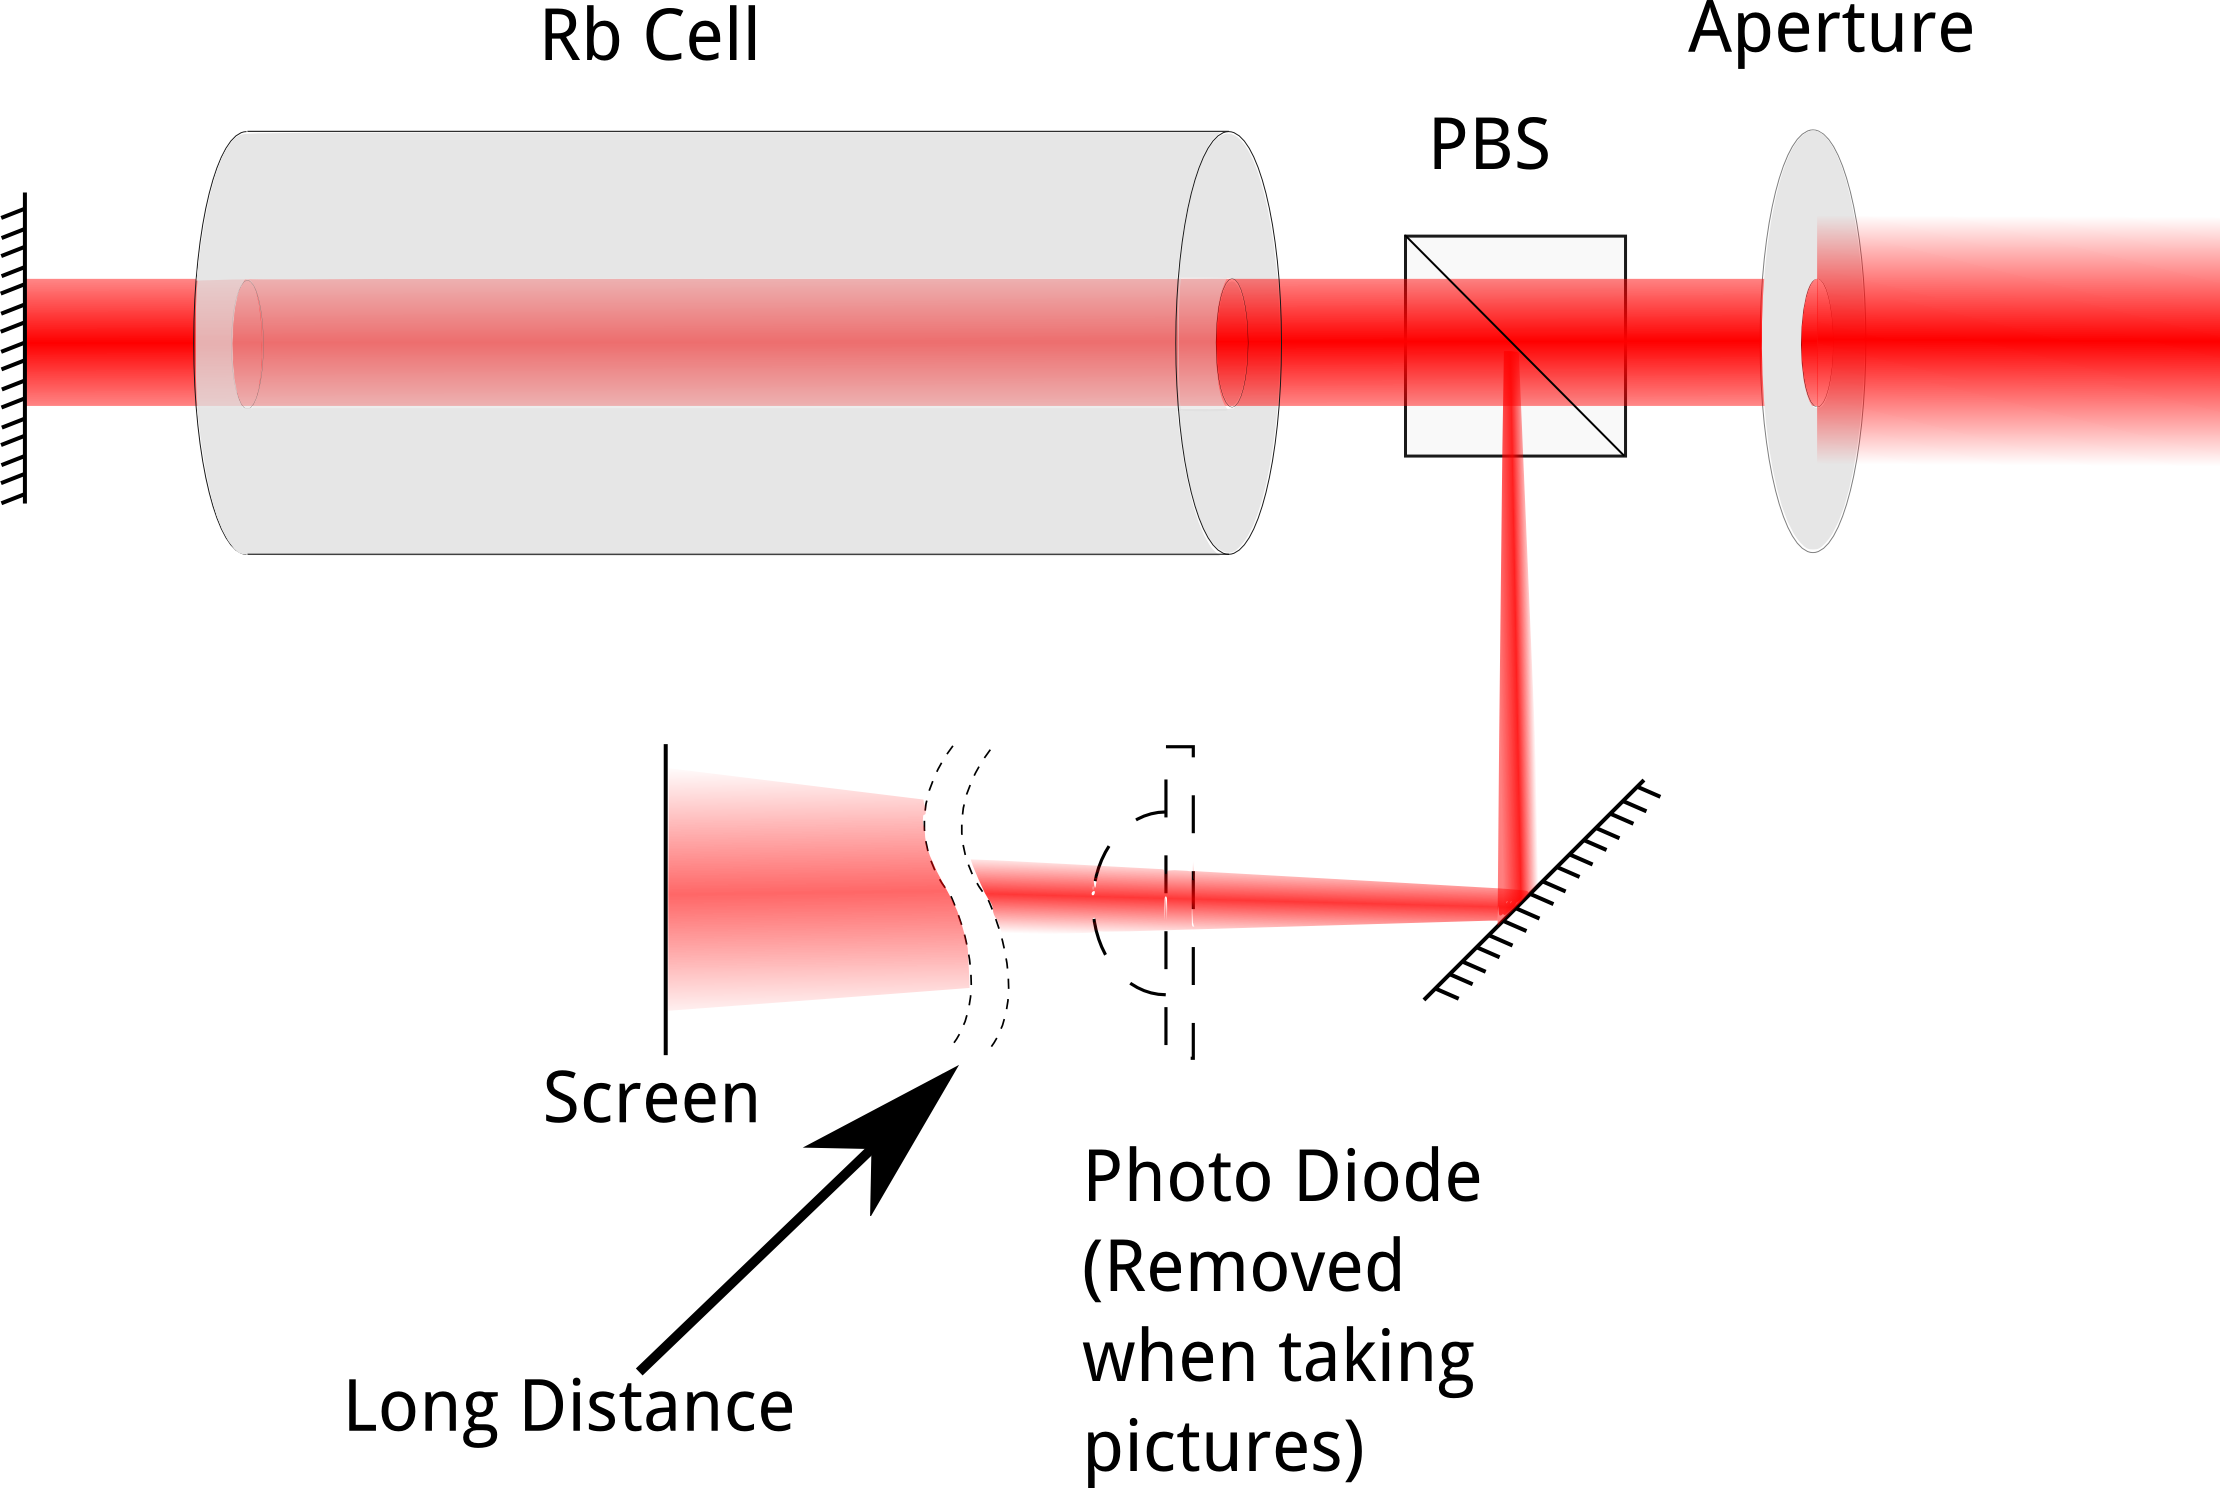
\includegraphics[width=9cm]{apparatus.png}
  \caption{}
  \label{apparatus}
\end{figure}
\subsection{Heater design.}
\subsection{Imaging system.}

\section{Measurements and results}
\subsection{Generated light in the orthogonal polarization.}
\begin{figure}
  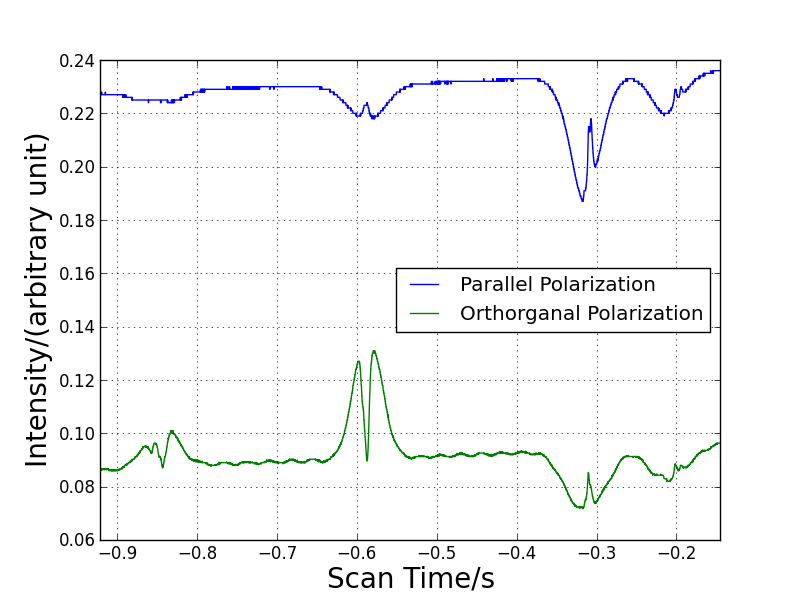
\includegraphics[width=9cm]{../data/5-16_csv/intensities.png}
  \caption{}
  \label{intensities}
\end{figure}

\subsection{Interference rings for red detuned light.}
\begin{figure}
  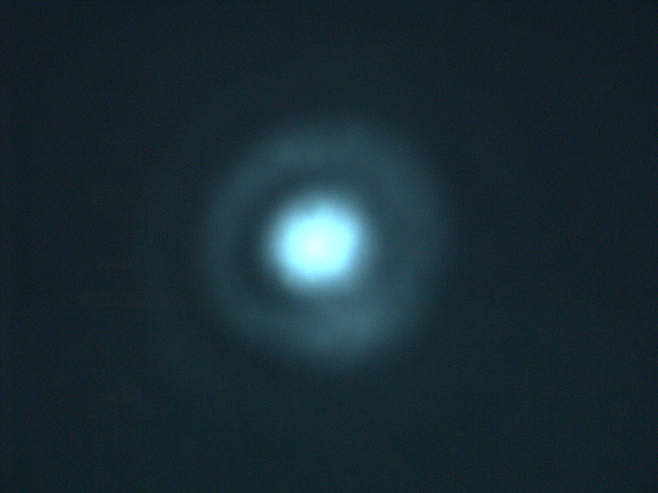
\includegraphics[width=7.8cm]{rings.png}
  \caption{}
  \label{rings}
\end{figure}
\begin{figure}
  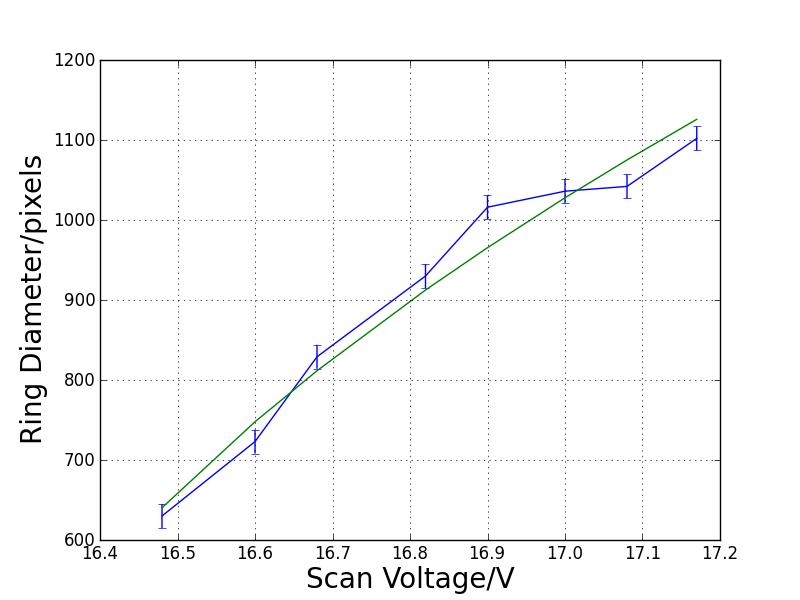
\includegraphics[width=9cm]{../data/5-16/ring-fit.png}
  \caption{}
  \label{ring_fit}
\end{figure}

\subsection{Flower like patterns}
\begin{figure}
  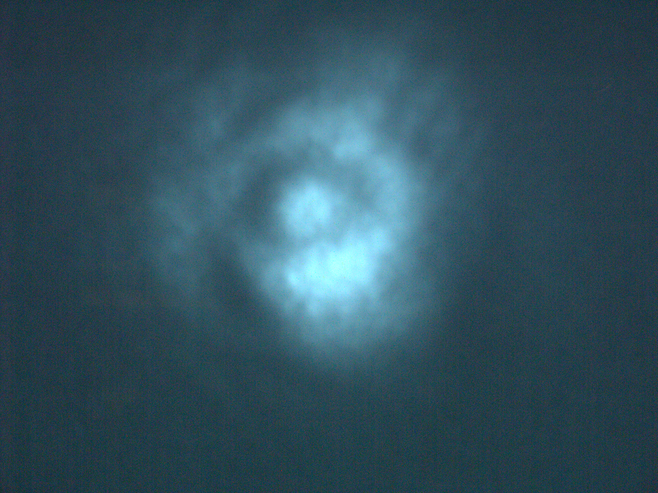
\includegraphics[width=7.8cm]{cone.png}
  \caption{}
  \label{cone}
\end{figure}
\begin{figure}
  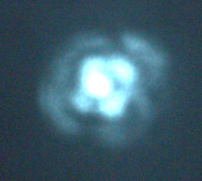
\includegraphics[width=7.8cm]{flower1.png}
  \caption{}
  \label{flower1}
\end{figure}
\begin{figure}
  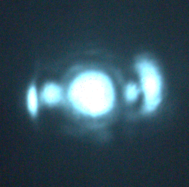
\includegraphics[width=7.8cm]{flower2.png}
  \caption{}
  \label{flower1}
\end{figure}
\begin{figure}
  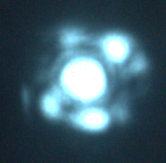
\includegraphics[width=7.8cm]{flower3.png}
  \caption{}
  \label{flower1}
\end{figure}

\section{Conclusion}

\bibliography{report}
\end{document}
